\documentclass{article}
\usepackage{graphicx}
\usepackage{amsmath}
\usepackage[parfill]{parskip}
\usepackage{hyperref}
\graphicspath{ {./figures/} }

\title{COMP.SEC.220 Security Protocol\footnote{github --- \url{https://github.com/ancuongnguyen07/SecurityProtocol}}}
\author{Cuong Nguyen --- LAB 5}
\date{27/09/2022}

\begin{document}
    
\maketitle

\section*{Task 1 --- Setting up two virtual machines}
%
\begin{figure}[!hpt]
    \centering
    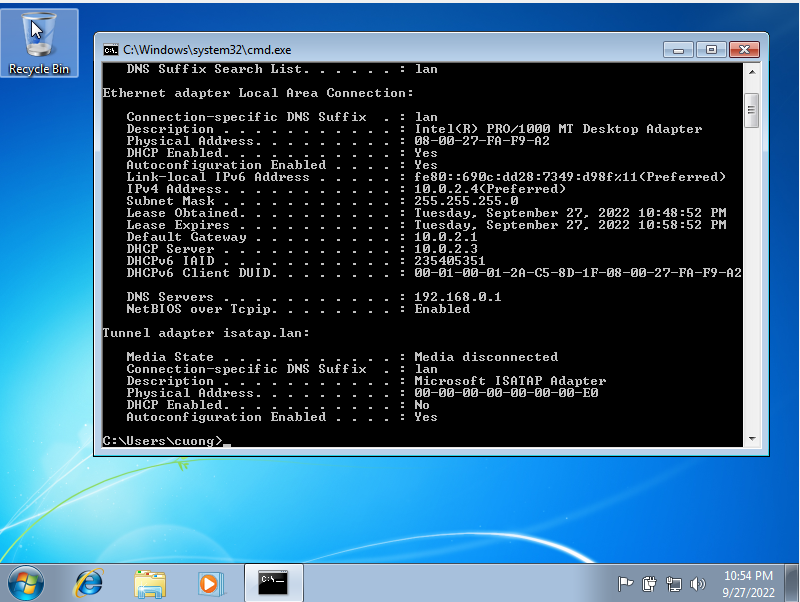
\includegraphics[width=\textwidth,height=\textheight,keepaspectratio]{win7_mac_ip.png}
    \caption{IP and MAC address of Windows virtual machine}
    \label{fig:win_mac_ip}
\end{figure}

As you can see in the \autoref{fig:win_mac_ip}, the Windows 7 virtual machine has:
\begin{itemize}
    \item IPv4 address: 10.0.2.4
    \item MAC address: 08-00-27-FA-F9-A2
    \item Default Gateway: 10.0.2.1
\end{itemize}

\begin{figure}[!hpt]
    \centering
    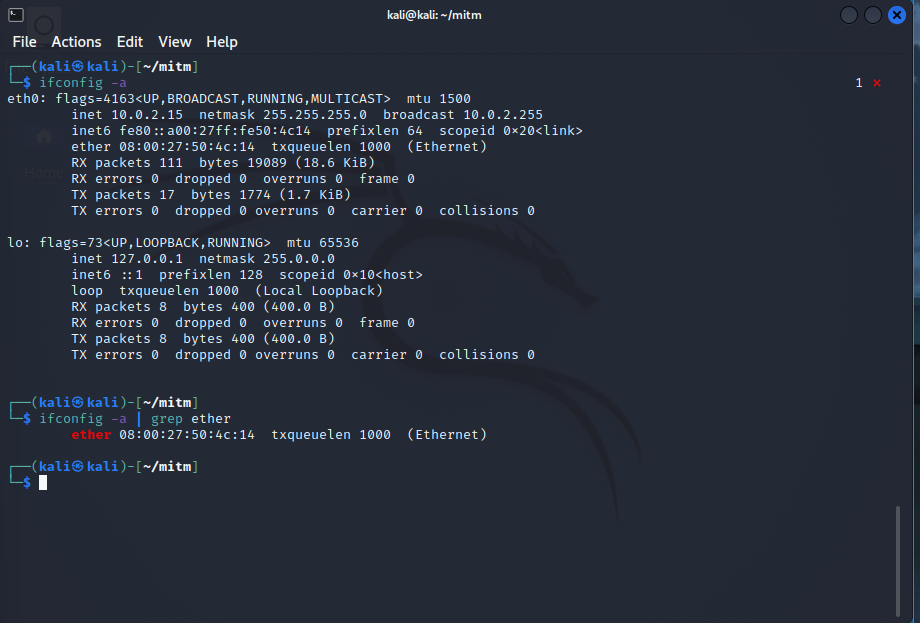
\includegraphics[width=\textwidth,height=\textheight,keepaspectratio]{kali_mac_ip.png}
    \caption{IP and MAC address of Kali Linux virtual machine}
    \label{fig:kali_mac_ip}
\end{figure}

As shown in the \autoref{fig:kali_mac_ip}, the Kali Linux virtual machine has:
\begin{itemize}
    \item IPv4 address: 10.0.2.15
    \item MAC address: 08:00:27:50:4c:14
\end{itemize}

\section*{Task 3 --- Testing the attack}
%
\begin{figure}[!hpt]
    \centering
    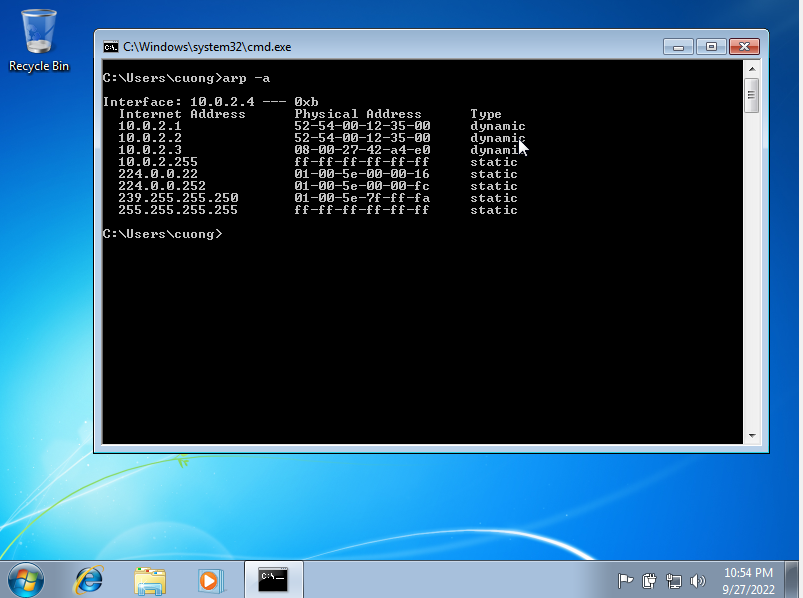
\includegraphics[height=\textheight,width=\textwidth,keepaspectratio]{win7_gateway_router_mac.png}
    \caption{MAC addresses of the default gateway on the Windows 7 virtual machine}
    \label{fig:router_dg_mac}
\end{figure}

As illustrated in the \autoref{fig:router_dg_mac}, the MAC address of the default gateway is
\textbf{52-54-00-12-35-00}. However, after the attack, the MAC address is changed into the
address of Kali Linux virtual machine, as shown in the \autoref{fig:poisonous_mac}

\begin{figure}[!hpt]
    \centering
    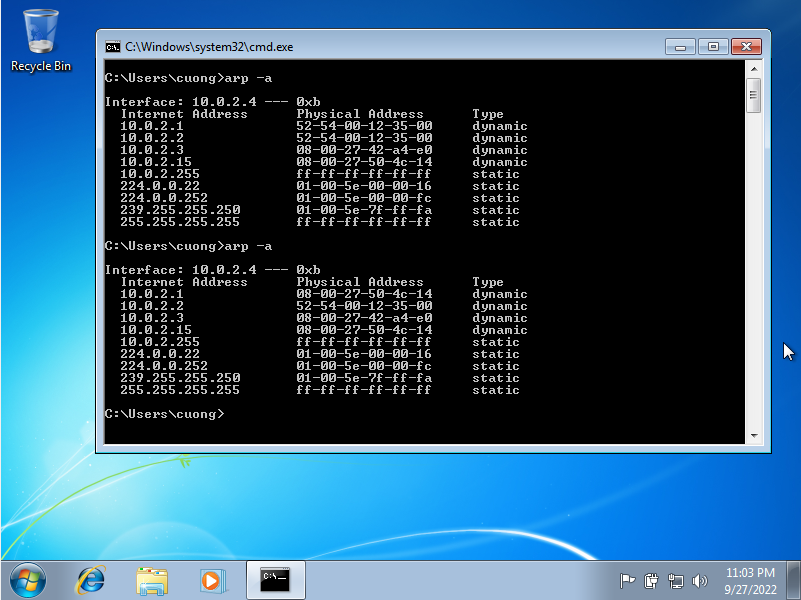
\includegraphics[width=\textwidth,height=\textheight,keepaspectratio]{arp_poisoned_mac.png}
    \caption{The poisonous MAC address of the default gateway on the Windows 7 virtual machine}
    \label{fig:poisonous_mac}
\end{figure}

\end{document}